%!TEX root = ../dokumentation.tex

%TODO: Einleitungen überarbeiten
\chapter{Projekt-Planung}\label{cha:Planung}
\section{Anforderungsanalyse}\label{sec:Anforderungsanalyse}
Basierend auf der grundlegenden Idee, eine Drohne mit Sensoren auszustatten, um damit die Luftqualität messen zu können, ist eine Anforderungsanalyse entstanden, welche die Funktionalitäten der ausgestatteten Drohne eindeutig spezifiziert. Die vollständige Anforderungsanalyse findet sich im Anhang.
\subsection{Muss-Kriterien}\label{subsec:MussKrit}
Im Folgenden werden zunächst die Kernanforderungen näher erläutert und warum diese absolute Priorität genießen.
\newline
\begin{enumerate}[label=\roman*.]
	\item Der Drohnenflug muss mittels der App gestartet werden können
	\item Die Flugroute muss mittels der App festgelegt werden können
	\item Der Drohnenflug muss mittels der App abgebrochen werden können
	\item Die Messwerte müssen über die App einsehbar sein
	\item Die Messwerte müssen über die App exportierbar sein
	\item Die App muss dem Benutzer ermöglichen, einen Flugbereich auf einer Karte zu markieren
	\item Die App muss dem Benutzer ermöglichen, die Flughöhe für die Messung auszuwählen
	\item Die auf der Karte ausgewählte Flugroute muss gestartet werden können
	\item Die App muss dem Benutzer ermöglichen, aus verschiedenen Messhäufigkeiten auszuwählen
	\item Die Drohne muss Feinstaub messen können (2.5 \& 10 $\mu m$)
	\item Die Drohne muss Druck messen können
	\item Die Drohne muss Feuchtigkeit messen können
	\item Die Drohne muss Temperatur messen können
	\item Die Drohne muss Stickoxide (NO\textsubscript{x}) messen können	
\end{enumerate}
Wie aus den obigen Anforderungen ersichtlich ist, liegt das Hauptaugenmerk darauf, die Drohne mittels einer App ansprechen und steuern zu können, während die Sensoren die gemessenen Umgebungsdaten an die App senden, damit diese dort angezeigt werden. Das Senden sowie das Verarbeiten der Sensordaten geschieht mittels des Bosch \acf{XDK}, welches als Schnittstelle zwischen den Sensoren und der App dient.
\subsection{Soll-Kriterien}\label{subsec:SollKrit}
In Ergänzung zu diesen kritischen Anforderungen, werden nachfolgend weitere Funktionalitäten beschrieben, welche ebenfalls für sinnvoll erachtet wurden, die jedoch nicht besonders kritisch sind. Die ergänzten Funktionalitäten umschließen weitere zu messende Größen sowie einige graphischen Verbesserungen, die eine übersichtlichere Rückmeldung zur laufenden Messung bieten sollen.
\newline
\begin{enumerate}[label=\roman*.]
	\item Die Messwerte sollen in der App visualisiert werden 	
	\item Die App soll die Messdaten in Abhängigkeit der Höhe zweidimensional auf der Karte anzeigen können
	\item Basierend auf dem auswählbaren Flugbereichs auf einer Karte, soll die App eine Flugroute automatisch berechnen können.
	\item Die App soll dem Benutzer ermöglichen, Bereiche explizit aus dem Flugbereich auszuschließen
	\item Die App soll die Drohnenposition während des Fluges auf einer Karte anzeigen
	\item Die App soll eine Fortschrittsanzeige zur laufenden Messung bieten
	\item Die App soll einen permanenten Video-Stream während des Drohnenflugs anzeigen
	\item Die Drohne soll Kohlenstoffdioxid (CO\textsubscript{2}) messen können
	\item Die Drohne soll Ozon (O\textsubscript{3}) messen können	
\end{enumerate}
\subsection{Kann-Kriterien}\label{subsec:KannKrit}
Sollten die oben genannten Funktionalitäten noch immer nicht den Rahmen des Projektes sprengen, sind mit den folgenden Anforderungen noch einige optionale Funktionalitäten erfasst, die potentiell einen weiteren Mehrwert liefern.
\newline
\begin{enumerate}[label=\roman*.]
	\item Der Benutzer kann in der App Flugrouten erstellen, speichern und abrufen 
	\item Der Benutzer kann in der App Messprofile erstellen, speichern und abrufen 
	\item Die App kann die Benutzerprofile exportieren können
	\item Die App kann durch Verrechnung von verbleibendem Akkustand und der vorgegebenen Flugroute einen Warnhinweis an den Benutzer geben, dass die Messung potenziell nicht ausgeführt werden kann
	\item Die App kann die Messdaten dreidimensional darstellen
	\item Die Drohne kann Kohlenstoffmonoxid (CO) messen können
	\item Die Drohne kann Schwefeldioxid (SO\textsubscript{2}) messen können
	\item Die Drohne kann flüchtige organische Verbindungen (VOC) messen können
	\item Die Drohne kann Methan (CH\textsubscript{4}) messen können	
	\item Der Anwender kann die Messdaten mittels der App einem Server übermitteln können	
\end{enumerate}
\section{Aufgabenteilung}\label{sec:Aufgabenteilung}
Um eine klare Trennung und Zuordnung der Aufgaben zu erreichen, ist das Projekt grob in 2 Bereiche eingeteilt. 
\newline
Die erste Komponente ist die iOS-App, welche für die Ansteuerung der Drohne, sowie die Visualisierung der Messdaten zuständig ist.
\newline
Die zweite Komponente ist der Entwurf des Messsystems mit allen Sensoren, deren Verschaltung und die Verarbeitung deren Daten mittels des Bosch \acs{XDK}.
\newline
\newline
Alle Aufgaben hinsichtlich der App werden von Julian Riegger bearbeitet, während alle Aufgaben zum Messsystem von Sebastian Breit bearbeitet werden.
\section{Zeitplan}\label{sec:Zeitplan}
In Ergänzung zu der bereits erwähnten Aufgabenteilung, wird zur besseren Planung und Nachverfolgung des Projektes ein Zeitplan verwendet, der auf einer hohen Abstraktionsebene die Aufgaben zeitlich einplant. Der Zeitplan ist mittels des frei verfügbaren Online-Tools Agantty erstellt, mit dessen Hilfe man einfach und unkompliziert Projekt-Pläne erstellen kann und dabei spezifische Aufgaben bestimmten Personen zuordnen kann. 
\newline 
\newline
Abbildung ~\ref{fig:Zeitplan} zeigt den erstellten Zeitplan.
\begin{figure}[H]
	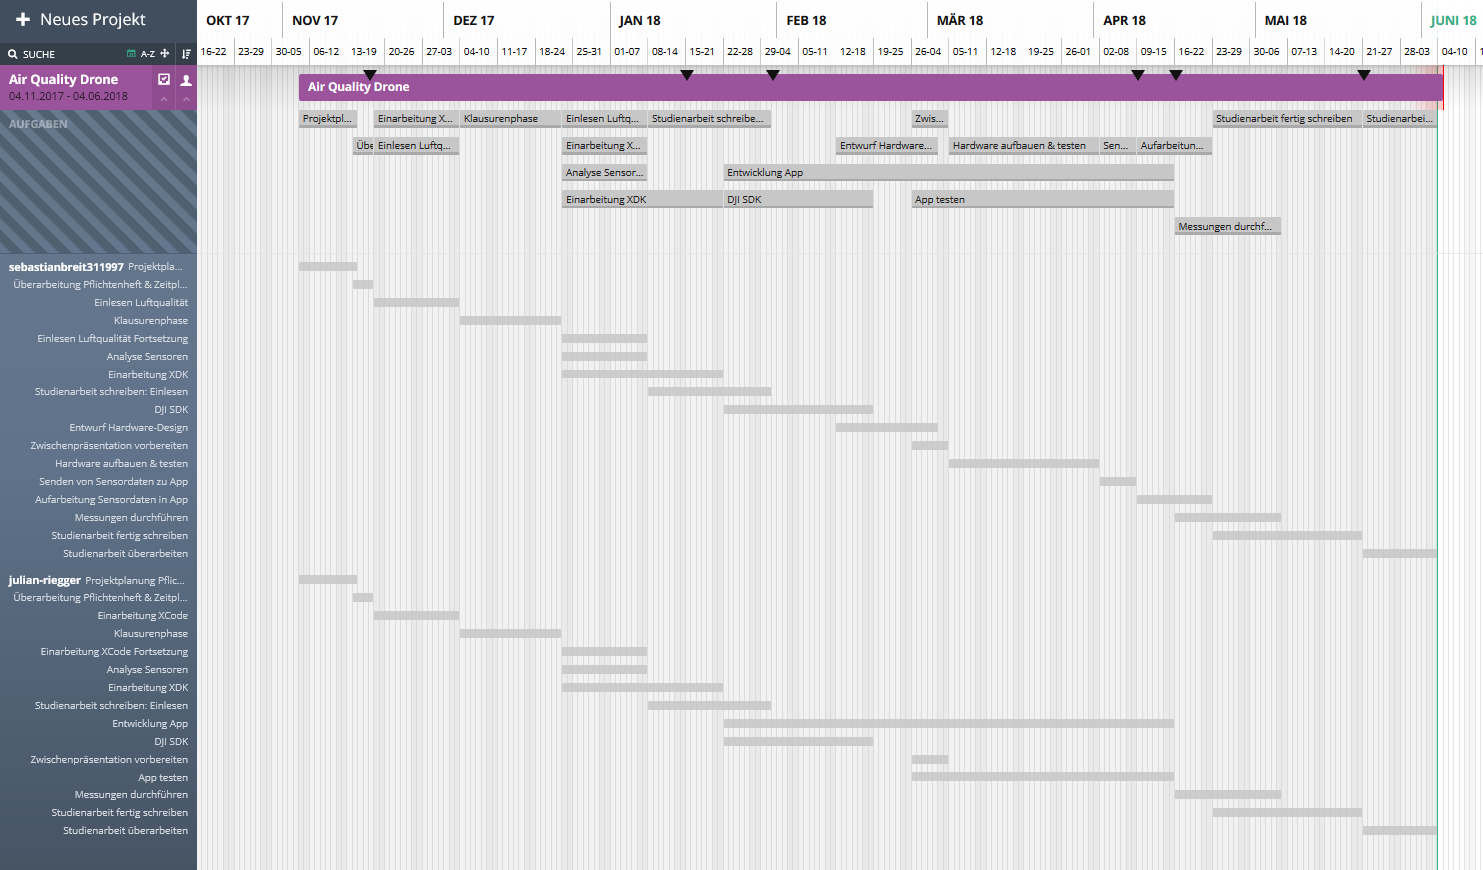
\includegraphics[width=\textwidth]{images/Zeitplan.png}	
	\caption{Zeitplan}
	\label{fig:Zeitplan}
\end{figure}


